\section{Experiments}

This section presents two experiments. The first one has been applied in an emulated component and The second experiment has been applied in an installed Moodle application. The experiments used this fitnesse function:

\begin{equation}
\begin{aligned}
fit=0.9* 90percentiletime\\
+0.1*80percentiletime\\+
0.1*70percentiletime+\\
0.1*maxResponseTime+\\
0.2*numberOfUsers-penalty
\end{aligned}
\end{equation}

The fitnesse function used in the experiments intended to find individuals with the highest percentile of 90\%, followed by individuals with higher percentile time of 80\% and 70\%, maximum response time and number of users.

The experiments have  emulated 27 generations with 300 executions by generation (100 times for each algorithm),  generating 300 news individuals. The experiments had used a initial population of 100 individuals. The Genetic Algorithm used the top 10 individuals from each generation to the crossover operation. The Tabu List has been configured with the size of 10 individuals and expire every 2 generations.  The mutation operation was applied to 10\% of the population on each generation. 

\subsection{First Experiment- Emulated Class Test}

The first experiment aimed to apply performance, load and stress testing in a simulated component. The purpose of using a simulated component is able to perform a greater number of generations in a shorter time available and eliminate variables such as the use of databases and application servers. The first experiment used a test class  named SimulateConcurrentAccess. These class have a static variable named \textit{x} and a set of methods that uses the variable in a synchronized context ( Listing \ref{classsimulated}).

\lstdefinestyle{outline}{
		language=Java,
         basicstyle=\scriptsize\ttfamily,
         numberstyle=\tiny,
         numbersep=5pt,
         tabsize=2,
         extendedchars=true,
         breaklines=true,
         keywordstyle=\color{black}\bf,
         frame=b,  % <<<<<<<<<<<<<<<<<<<<<<<<<<
         stringstyle=\color{green!40!black}\ttfamily,
         showspaces=false,
         showtabs=false,
         numbers=left,
         xleftmargin=17pt,
         framexleftmargin=17pt,
         framextopmargin=1pt, % <<<<<<<<<<<<<<<<<<<<<<
         showstringspaces=false,
         %backgroundcolor=\color[RGB]{200,200,200},
         belowcaptionskip=0pt
}

\begin{lstlisting}[style=outline,caption={SimulateConcurrentAcess class},label=classsimulated]
public class SimulateConcurrentAccess {
  @Test
  public void test() {		
    synchronized (StaticClass.class) {
			for (int i = 0; i <= 1000; i++) {
				StaticClass.x += i;
			}
			StaticClass.x = 0;
		}
	}
\end{lstlisting}


Fig.\ref{fig:exp1bestresults} presents the best results in 27 generations applied in the first experiment . The Figure shows the results obtained with the algorithms with and without collaboration. The $x$ axis  represents the generation number and the $y$ axis represents the best fitnesse value obtained until the current generation. The results of the experiment showed that the use of cooperation between the three algorithms resulted in find individuals with better fitnesse values.

\begin{figure}[h]
\centering
\caption{Best results obtained in 27 generations}
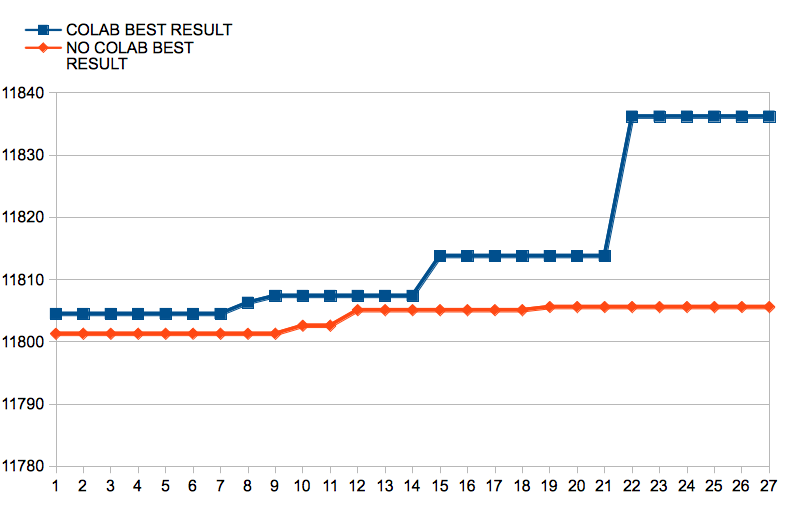
\includegraphics[width=0.5\textwidth]{./images/exp1bestresults.png}
\label{fig:exp1bestresults}
\end{figure}
The table \ref{tab:averagefirst} presents the results obtained by Genetic Algorithm (GA) and TABU Search (TS) from 27 generations in the first experiment. The four columns of the table represent the use of GA a TS with collaboration  (Col) and with no collaboration (No).  The values are the average of the fitnesse value obtained by each algorithm. 

\begin{table}[h]
\centering
\caption{Fitnesse function Average  by algorithm in the first experiment }
\label{tab:averagefirst}
\begin{tabular}{|l|l|l|l|l|}
\hline
G & GA Col  & GA No & TS Col  & TS No\\ \hline
1 & 2855 & 2855 & 2855.00 & 2855\\ \hline
2 & 9545 & 9245 & 10714 & 10591\\ \hline
3 & 9346 & 5535 & 10718 & 8932\\ \hline
4 & 3827 & 5957 & 8527 & 3000\\ \hline
5 & 5880 & 10738 & 8527 & 3000\\ \hline
6 & 11801 & 9583 & 8797 & 8650\\ \hline
7 & 4984 & 9241 & 9985 & 4139\\ \hline
8 & 9063 & 10085 & 9985 & 5256\\ \hline
9 & 8915 & 9099 & 9998 & 6779\\ \hline
10 & 9945 & 10281 & 10163 & 6832\\ \hline
11 & 9991 & 8831 & 10352 & 9048\\ \hline
12 & 10535 & 10578 & 10425 & 9819\\ \hline
13 & 10325 & 10383 & 10319 & 9652\\ \hline
14 & 11414 & 7197 & 9948 & 9394\\ \hline
15 & 10754 & 7189 & 10388 & 1701\\ \hline
16 & 10632 & 7309 & 9878 & 4193\\ \hline
17 & 10108 & 8762 & 10007 & 5300\\ \hline
18 & 4769 & 8360 & 10007 & 5430\\ \hline
19 & 7397 & 9527 & 5508 & 5716\\ \hline
20 & 8418 & 10378 & 4816 & 7417\\ \hline
21 & 9526 & 10301 & 9243 & 8940\\ \hline
22 & 7128 & 9595 & 8095 & 9872\\ \hline
23 & 8519 & 9981 & 9332 & 11024\\ \hline
24 & 10053 & 9647 & 10138 & 9479\\ \hline
25 & 8759 & 11045 & 9313 & 10668\\ \hline
26 & 9601 & 10798 & 8629 & 10837\\ \hline
27 & 6352 & 10739 & 10367 & 9754\\ \hline
\end{tabular}
\end{table}

The signed-rank Wilcoxon non-parametrical procedure was used for comparing the results. The test showed that there was no significant improvement in the use of collaborative approach to the use of genetic algorithms. However , the use of collaborative approach showed significant improvement in the use of the algorithm TS and in turn the final result obtained.

\begin{lstlisting}[style=outline,caption={Result obtained by the  Wilcoxon test with the results of TS Colab and TS No},float,label=classsimulated]

Result Details

W-value: 70
Mean Difference: -1497.04
Sum of pos. ranks: 281
Sum of neg. ranks: 70

Z-value: -2.6795
Mean (W): 175.5
Standard Deviation (W): 39.37

Sample Size (N): 27

Result 1 - Z-value

The Z-value is -2.6795. The p-value is 0.00736. The result is significant at p≤ 0.05.

Result 2 - W-value

The W-value is 70. The critical value of W for N = 26 at p≤ 0.05 is 98. Therefore, the result is significant at p≤ 0.05.
\end{lstlisting}


\subsection{Second Experiment- Moodle Application Test}

The second experiment uses a Moodle application installed in a machine with 500 Gb of hard disk and 8 Gb of memory.The study used six application scenarios:

\begin{itemize}
\item PostDeleteMessage- This scenario post and delete messages in the moodle application.
\item MyHome- This scenario access the user's homepage of the application.
\item Login- This scenario are responsible by the user authentication of the application.
\item Notifications- This scenario enter in the notification page of each user.
\item Start Page- Initial start page of the application.
\item Badge- This scenario enter in the Badge page.
\end{itemize}

The maximum tolerated response time in test was 30 seconds.  Any  individuals that obtained a time longer than the stipulated maximum time suffered penalties.  The whole process of stress and performance tests, which took three days and about 1800 executions, was carried out without the need for monitoring of a test designer. The tool have  selected automatically the next scenarios to be run up to the limit of six generations previously established. 

The Fig. \ref{fig:g13moodle} presents the resume of the results obtained in the six generations of the experiment. The results are grouped by algorithm type (colaboration or non colaboration) and generation.  The columns presents the fitnesse average value by each algorithm. The results of the experiment showed that The TABU search algorithm found most of the best individuals. The use of cooperation between the three algorithms resulted in better fitnesse values in most experiments. The experiment succeeded in finding 29 individuals where the maximum time expected by the application was obtained.  The Fig. \ref{fig:individuals} has four individuals who have obtained the maximum time expected by the application.

\begin{figure}[h]
\centering
\caption{Example of individuals obtained in the second experiment}
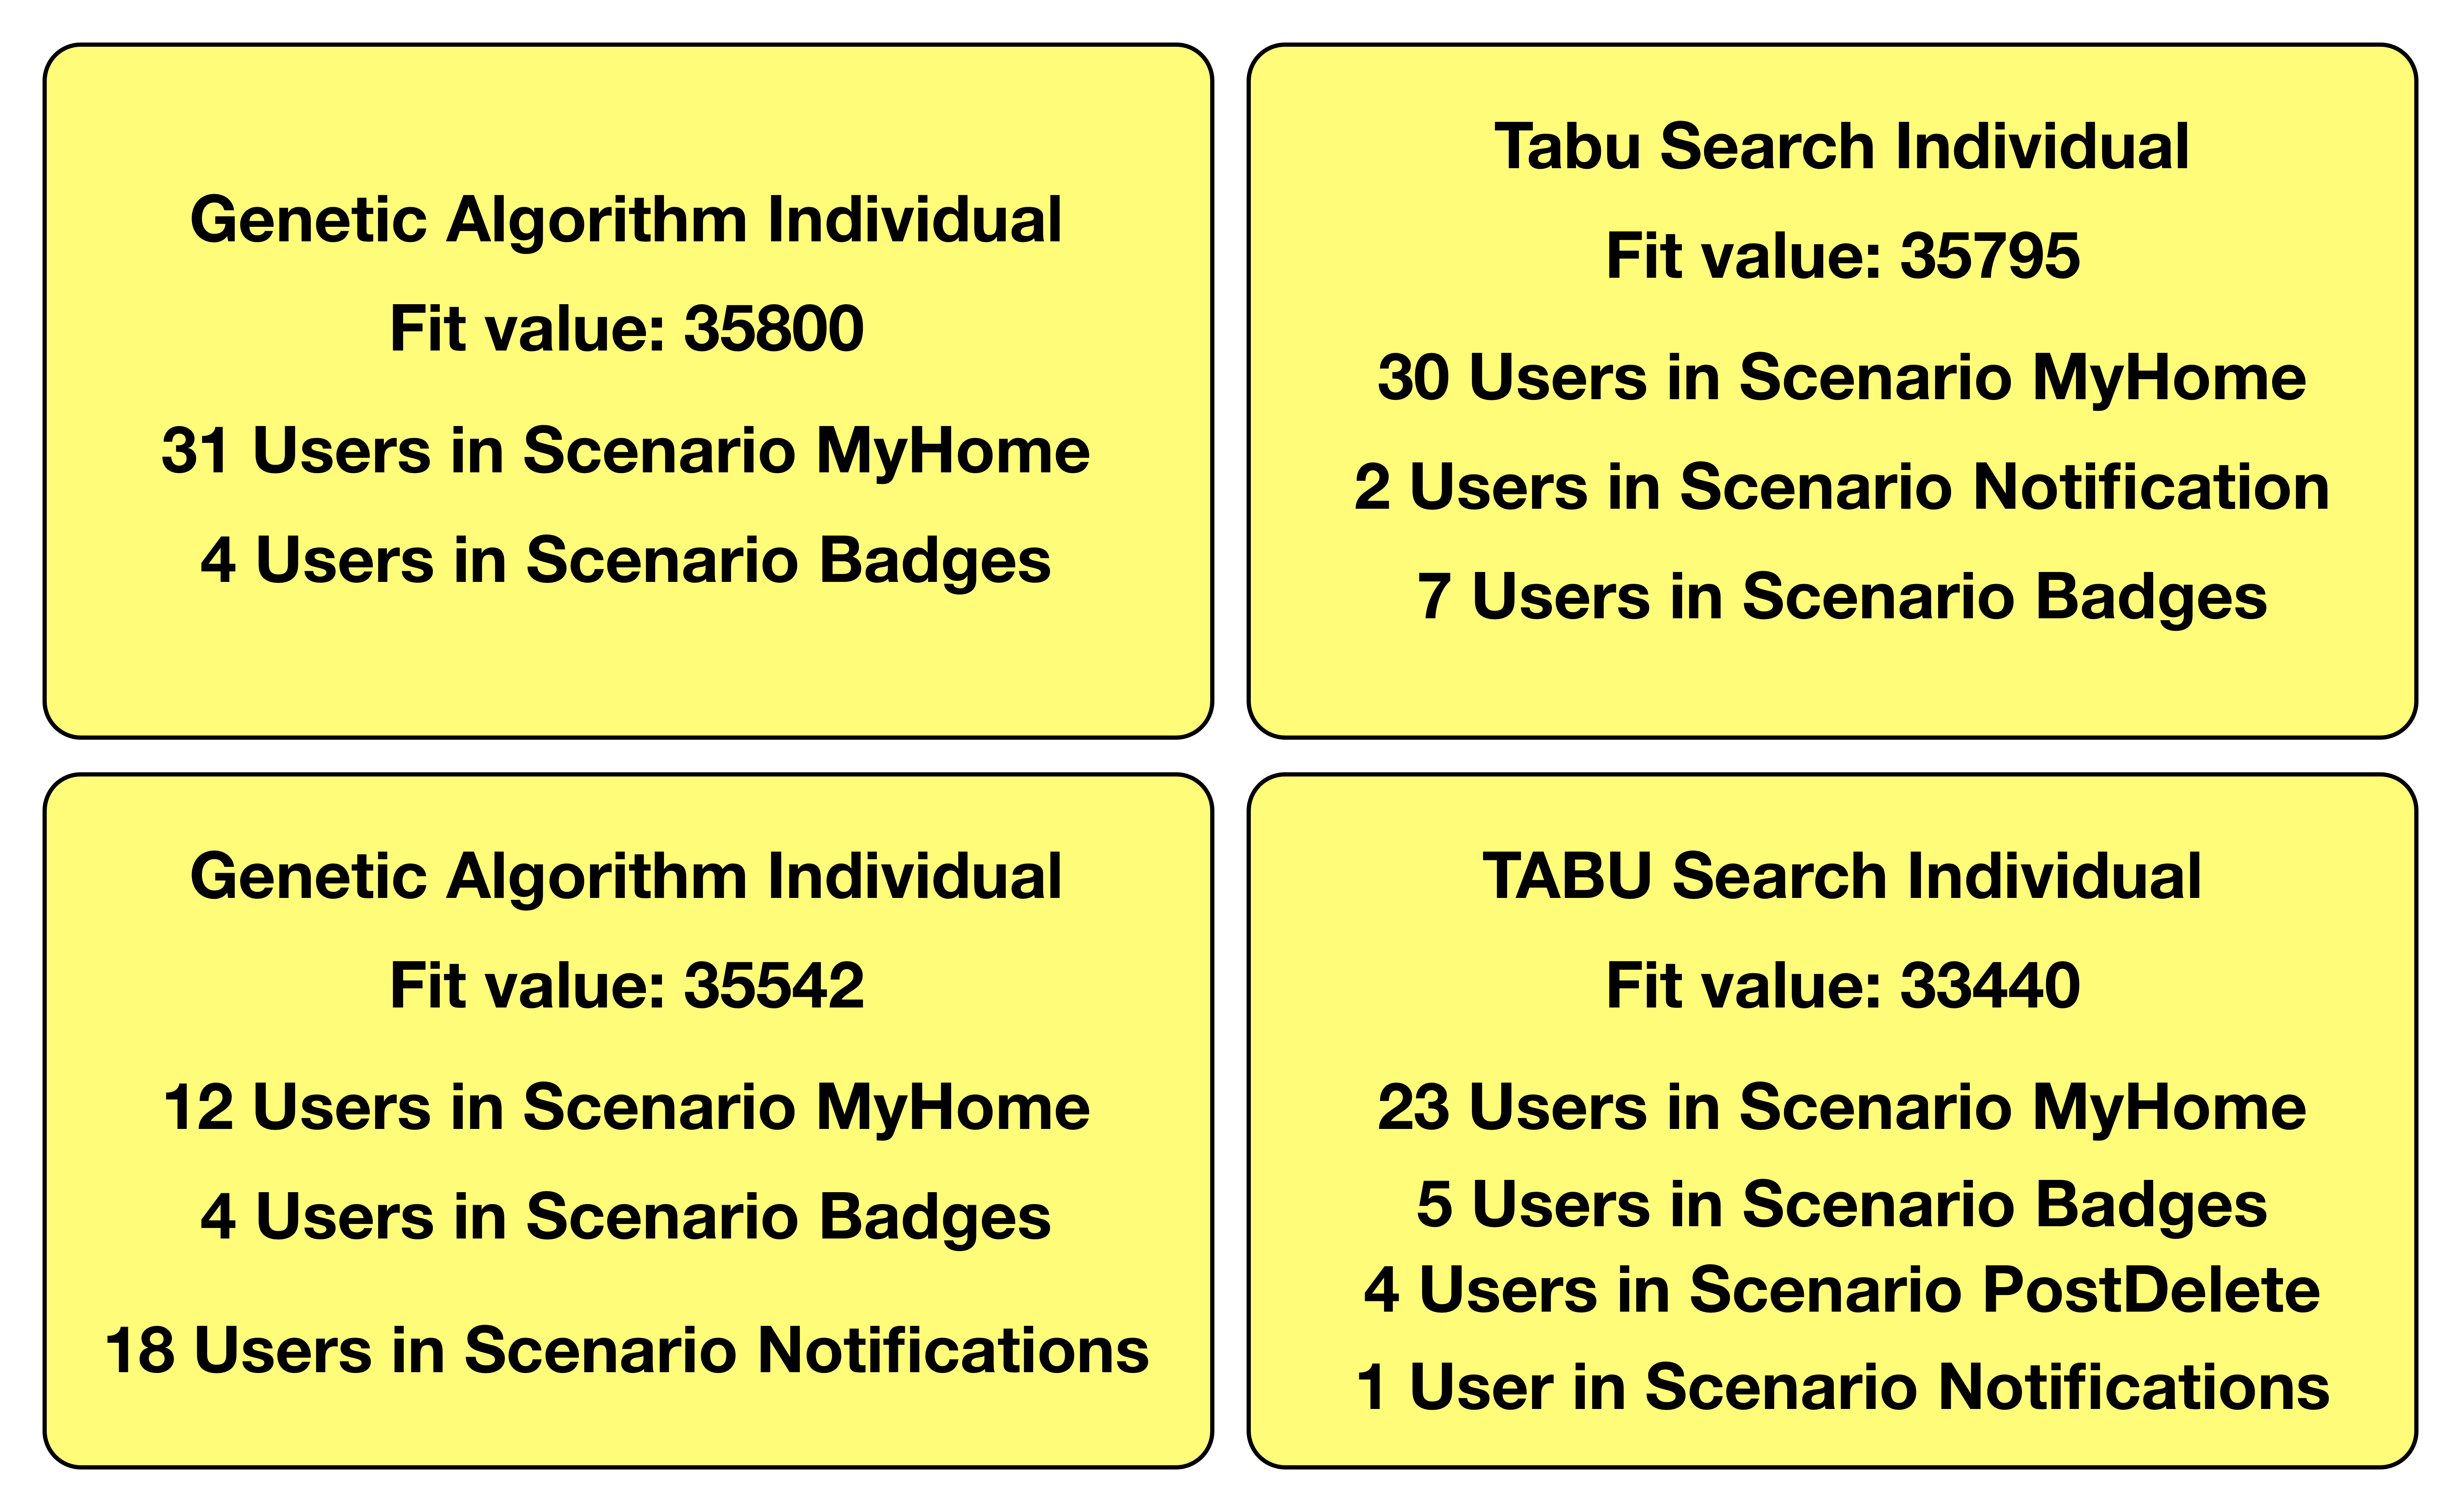
\includegraphics[width=0.5\textwidth]{./images/individuals.png}
\label{fig:individuals}
\end{figure}

\begin{figure*}[h]
\centering
\captionof{figure}{The results for the first generations (1-6) of tests applied in the Moodle application}
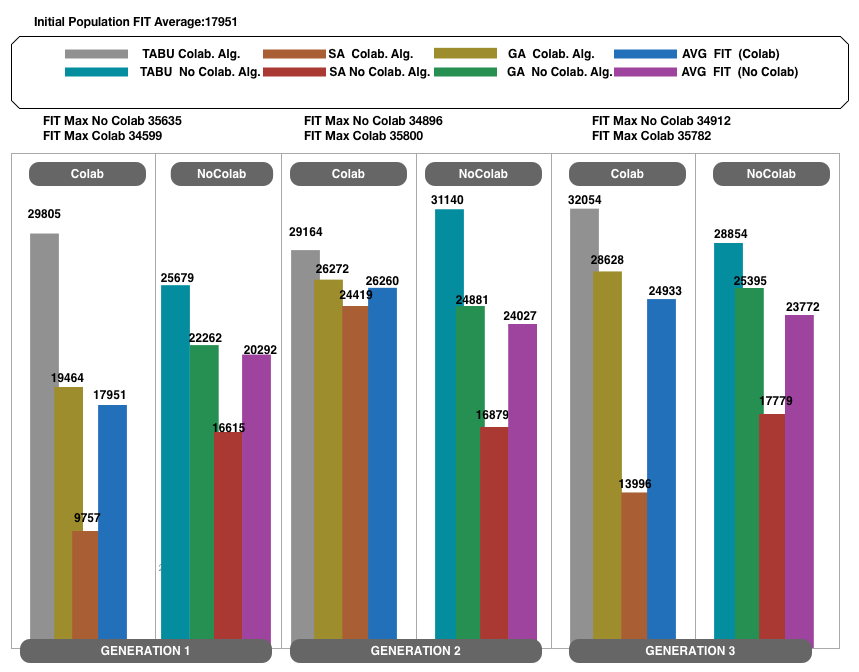
\includegraphics[width=0.8\textwidth]{./images/GENERATIONS1.png}
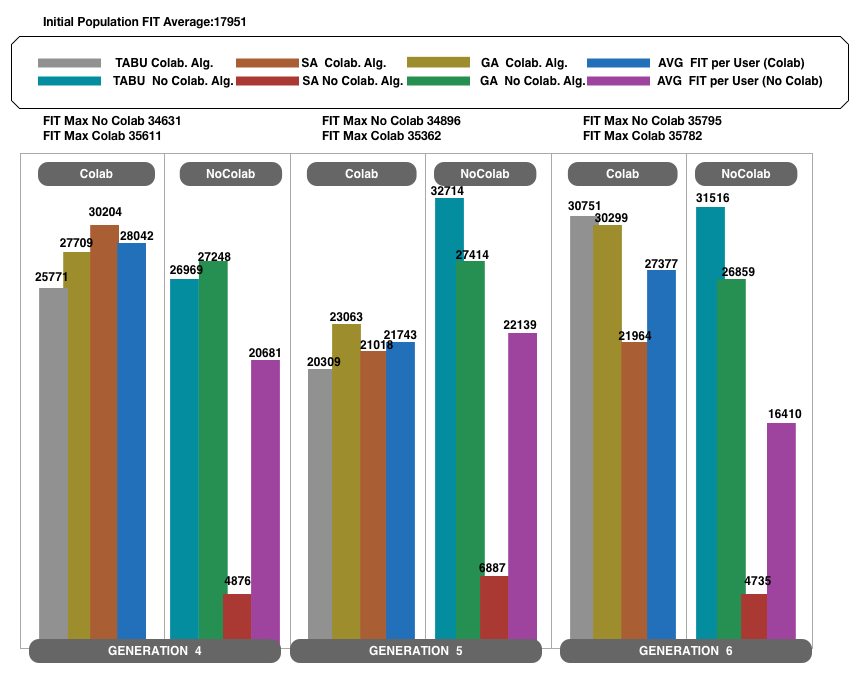
\includegraphics[width=0.8\textwidth]{./images/GENERATIONS2.png}
\label{fig:g13moodle}
\end{figure*}
